
\begin{figure}[h!]
\begin{center}
\resizebox{0.5\textwidth}{!}
{
\begin{pspicture}(0,-2.0159376)(15.188437,2.0159376)
\psline[linewidth=0.04cm](0.1684375,-1.0303125)(15.168438,-1.0303125)
\psline[linewidth=0.04cm,arrowsize=0.05291667cm 2.0,arrowlength=1.4,arrowinset=0.4]{->}(3.1684375,0.9696875)(3.1684375,-1.0303125)
\psline[linewidth=0.04cm,arrowsize=0.05291667cm 2.0,arrowlength=1.4,arrowinset=0.4]{->}(6.1684375,-0.0303125)(6.1684375,-1.0303125)
\psline[linewidth=0.04cm,arrowsize=0.05291667cm 2.0,arrowlength=1.4,arrowinset=0.4]{->}(9.168438,-0.0303125)(9.168438,-1.0303125)
\psline[linewidth=0.04cm,arrowsize=0.05291667cm 2.0,arrowlength=1.4,arrowinset=0.4]{->}(12.168438,0.9696875)(12.168438,-1.0303125)
\psline[linewidth=0.04cm](6.1684375,-0.0303125)(7.4684377,-0.0303125)
\psline[linewidth=0.04cm](7.9684377,-0.0303125)(9.168438,-0.0303125)
\psline[linewidth=0.04cm](3.1684375,0.9696875)(8.168438,0.9696875)
\psline[linewidth=0.04cm](9.168438,0.9696875)(12.168438,0.9696875)
\pscircle[linewidth=0.04,dimen=outer](7.7184377,0.0196875){0.25}
\pscircle[linewidth=0.04,dimen=outer](8.668438,0.9696875){0.5}
\psline[linewidth=0.04cm,arrowsize=0.05291667cm 2.0,arrowlength=1.4,arrowinset=0.4]{->}(7.4684377,-0.2303125)(8.068438,0.3696875)
\psline[linewidth=0.04cm,arrowsize=0.05291667cm 2.0,arrowlength=1.4,arrowinset=0.4]{->}(8.168438,0.4696875)(9.268437,1.6696875)
\usefont{T1}{ptm}{m}{n}
\rput(7.9475,-0.4553125){\LARGE $\Delta U$}
\usefont{T1}{ptm}{m}{n}
\rput(7.974375,1.7446876){\LARGE Source $I$}
\usefont{T1}{ptm}{m}{n}
\rput(3.179375,-1.4553125){\LARGE A}
\usefont{T1}{ptm}{m}{n}
\rput(6.223906,-1.4553125){\LARGE M}
\usefont{T1}{ptm}{m}{n}
\rput(9.084687,-1.4553125){\LARGE N}
\usefont{T1}{ptm}{m}{n}
\rput(12.147187,-1.4553125){\LARGE B}
\usefont{T1}{ptm}{m}{n}
\rput(1.4175,-1.7553124){\LARGE $\rho$}
\usefont{T1}{ptm}{m}{n}
\rput(1.5075,-0.4553125){\LARGE $\rho=\infty$}
\end{pspicture} 
}

\caption{Four point measurement}
\label{fig:dc01}
\end{center}
\end{figure}
Resistivity $\rho$ of the subsurface derived from $I$ (which is known), $\Delta U$ (which is measured) and the geometrical factor $K$ (which is also known).

\subsubsection*{Frequently used electrode arrays}

\begin{figure}[h!]
\begin{center}
\includegraphics[width=0.5\textwidth]{Wenner.png}
a)
\includegraphics[width=0.5\textwidth]{Schlumberger.png}
b)
\includegraphics[width=0.5\textwidth]{Dipoldipol.png}
c)
\caption{a) Wenner, Half-Wenner; b) Schlumberger, Half-Schlumberger; c) Dipole-dipole, source???}
\label{fig:dc02}
\end{center}
\end{figure}

Industrial standard of measuring is via an \textit{Multielectrode array}.


\subsection{Basic equations of DC-resistivity}
The first assumption of DC-resistivity methods and the major difference to EM-methods is the assumption of stationary currents:
\begin{align*}
\frac{\partial}{\partial t}=0
\end{align*}
The fields do not depend on time.

Looking at the \textit{Maxwell's equations}:
\begin{align}
\nabla\times\vec{E}=\frac{\partial \vec{B}}{\partial t}=0
\end{align}
This means irrotational electric field and from that follows, that the electric field vector can be derived by a scalar potential:

\begin{equation}
\vec{E}=-\nabla V \label{eq:2-2}
\end{equation}
Insert equation \eqref{eq:2-2} into eq. \eqref{eq:1-2}:

\begin{equation}
\vec{j}=-\sigma \nabla V\label{eq:2-3}
\end{equation}
\textit{Continuity equation:}
\begin{equation}
\nabla\cdot\vec{j}+\frac{\partial q}{\partial t}=0
\end{equation}
Now new charges are generated in the course of time
\begin{equation}
\nabla\cdot\vec{j}=0 \label{eq:2-5}
\end{equation}
which is valid outside of the source.

If we insert eq. \eqref{eq:2-3} into \eqref{eq:2-5}:
\begin{align*}
-\nabla\cdot(\sigma\nabla V)&=0\\
\nabla\sigma\nabla V + \sigma\nabla^2V&=0
\end{align*}
$\nabla\sigma=0$ for areas with constant conductivity, so:
\begin{equation}
\nabla^2 V=0\label{eq:lapleq}
\end{equation}
which is called the \textit{Laplace-equation}, the basic equation of DC-resistivity.

Derivation of solutions of this elliptic partial differential equation using  different boundary conditions:

Assume a current source with strength $I$ at point $\vec{r}_0$, then the spatial current distribution can be given as:$\nabla\cdot\vec{j}=I\delta(\vec{r}-\vec{r}_0$
and so:
\begin{equation}
\nabla\cdot(\sigma\nabla V)=-I\delta(\vec{r}-\vec{r}_0)
\end{equation}
This equation can be solved numerically for arbitrary distribution of conductivity ratio.


\subsubsection{Potential of a current electrode}

\begin{figure}[h!]
\begin{center}
\resizebox{0.5\textwidth}{!}
{
\begin{pspicture}(0,-3.02)(10.189688,1.02)
\psline[linewidth=0.04cm](0.0,0.0)(8.0,0.0)
\rput{-180.0}(8.0,0.0){\psarc[linewidth=0.04,linestyle=dashed,dash=0.16cm 0.16cm](4.0,0.0){3.0}{0.0}{180.0}}
\psline[linewidth=0.04cm,arrowsize=0.05291667cm 2.0,arrowlength=1.4,arrowinset=0.4]{->}(4.0,1.0)(4.0,0.0)
\psline[linewidth=0.04cm,arrowsize=0.05291667cm 2.0,arrowlength=1.4,arrowinset=0.4]{->}(4.0,0.0)(1.2,-1.0)
\psline[linewidth=0.04cm,arrowsize=0.05291667cm 2.0,arrowlength=1.4,arrowinset=0.4]{->}(4.0,0.0)(4.0,-3.0)
\psline[linewidth=0.04cm,arrowsize=0.05291667cm 2.0,arrowlength=1.4,arrowinset=0.4]{->}(4.0,0.0)(6.9,-1.0)
\psline[linewidth=0.04cm,arrowsize=0.05291667cm 2.0,arrowlength=1.4,arrowinset=0.4]{->}(4.0,0.0)(1.7,-1.9)
\psline[linewidth=0.04cm,arrowsize=0.05291667cm 2.0,arrowlength=1.4,arrowinset=0.4]{->}(4.0,0.0)(6.3,-1.9)
\psline[linewidth=0.04cm,arrowsize=0.05291667cm 2.0,arrowlength=1.4,arrowinset=0.4]{->}(4.0,0.0)(2.7,-2.7)
\psline[linewidth=0.04cm,arrowsize=0.05291667cm 2.0,arrowlength=1.4,arrowinset=0.4]{->}(4.0,0.0)(5.3,-2.7)
\usefont{T1}{ptm}{m}{n}
\rput(8.788125,-0.595){equipotential surface}
\usefont{T1}{ptm}{m}{n}
\rput(2.1721876,-0.195){current flow}
\psline[linewidth=0.04cm,arrowsize=0.05291667cm 2.0,arrowlength=1.4,arrowinset=0.4]{->}(7.2,-0.6)(7.0,-0.5)
\psline[linewidth=0.04cm,arrowsize=0.05291667cm 2.0,arrowlength=1.4,arrowinset=0.4]{->}(1.7,-0.4)(1.8,-0.7)
\rput{-180.0}(8.0,0.0){\psarc[linewidth=0.04,linestyle=dashed,dash=0.16cm 0.16cm](4.0,0.0){2.0}{0.0}{180.0}}
\end{pspicture} 
}
\caption{Single current source}
\label{fig:singlesource}
\end{center}
\end{figure}

Using \textit{Ohm's law}: $\vec{E}=\rho\vec{j}=\rho\frac{I}{2\pi r^2}$, where $2\pi r^2$ is the surface of the half sphere. Using $E=-\frac{dV}{dr}$ follows the potential of a homogeneous half space:
\begin{equation}
V=\frac{\rho I}{2\pi r}
\end{equation}

\begin{figure}[h!]
\begin{center}
\resizebox{0.5\textwidth}{!}
{
\begin{pspicture}(0,-2.9690626)(13.175938,2.9890625)
\psline[linewidth=0.04cm](0.0,1.0509375)(8.0,1.0509375)
\psline[linewidth=0.04cm](2.0,-1.9490625)(4.0,2.0509374)
\psline[linewidth=0.04cm](4.0,2.0509374)(5.2,2.0509374)
\psline[linewidth=0.04cm](6.0,2.0509374)(6.8,2.0509374)
\psline[linewidth=0.04cm,linestyle=dashed,dash=0.16cm 0.16cm,arrowsize=0.05291667cm 2.0,arrowlength=1.4,arrowinset=0.4]{->}(6.8,2.0509374)(9.3,2.0509374)
\usefont{T1}{ptm}{m}{n}
\rput(10.955313,2.3959374){\Large $c_2\rightarrow\infty$}
\psdots[dotsize=0.16](2.0,-1.9490625)
\psline[linewidth=0.04cm,arrowsize=0.05291667cm 2.0,arrowlength=1.4,arrowinset=0.4]{->}(2.0,-1.9490625)(3.0,-1.9490625)
\psline[linewidth=0.04cm,arrowsize=0.05291667cm 2.0,arrowlength=1.4,arrowinset=0.4]{->}(2.0,-1.9490625)(2.0,-0.9490625)
\psline[linewidth=0.04cm,arrowsize=0.05291667cm 2.0,arrowlength=1.4,arrowinset=0.4]{->}(2.0,-1.9490625)(1.0,-1.9490625)
\psline[linewidth=0.04cm,arrowsize=0.05291667cm 2.0,arrowlength=1.4,arrowinset=0.4]{->}(2.0,-1.9490625)(2.0,-2.9490626)
\pscircle[linewidth=0.04,linestyle=dashed,dash=0.16cm 0.16cm,dimen=outer](2.0,-1.9490625){1.0}
\psline[linewidth=0.04cm,arrowsize=0.05291667cm 2.0,arrowlength=1.4,arrowinset=0.4]{->}(2.0,-1.9490625)(2.7,-2.6490624)
\psline[linewidth=0.04cm,arrowsize=0.05291667cm 2.0,arrowlength=1.4,arrowinset=0.4]{->}(2.0,-1.9490625)(1.3,-2.6490624)
\psline[linewidth=0.04cm,arrowsize=0.05291667cm 2.0,arrowlength=1.4,arrowinset=0.4]{->}(2.0,-1.9490625)(1.3,-1.2490625)
\psline[linewidth=0.04cm,arrowsize=0.05291667cm 2.0,arrowlength=1.4,arrowinset=0.4]{->}(2.0,-1.9490625)(2.7,-1.3490624)
\usefont{T1}{ptm}{m}{n}
\rput(3.5653124,-1.7040625){\Large $c_1$}
\pscircle[linewidth=0.04,dimen=outer](5.6,2.0509374){0.4}
\psline[linewidth=0.04cm,arrowsize=0.05291667cm 2.0,arrowlength=1.4,arrowinset=0.4]{->}(5.3,1.6509376)(6.0,2.5509374)
\usefont{T1}{ptm}{m}{n}
\rput(5.6876564,2.7809374){\large Source}
\end{pspicture} 
}

\caption{Mise-\`a-la-Masse method}
\label{fig:misemasse}
\end{center}
\end{figure}

In the case of the \textit{Mise-\`a-la-Masse method} the potential of the homogeneous full space is:
\begin{equation}
V=\frac{\rho I}{4\pi r}
\end{equation}

The same result can be derived by using the Laplace-equation \eqref{eq:lapleq} and the use of spherical coordinates:
\begin{align*}
\nabla^2 V=\frac{d^2V}{dr^2}+\frac{2}{r}\frac{dV}{dr}
\end{align*}
From the symmetry of the system the potential is a function of the distance to the source $r$ only. Multiplying by $r^2$ and integrating, we get:
\begin{align*}
\frac{dV}{dr}=\frac{c_1}{r^2}
\end{align*}
Integrating over $r$ again leads to the solution:
\begin{align*}
V=-\frac{c_1}{r}+c_2 && c_1,c_2 = const.
\end{align*}
To determine the constants we have to use boundary conditions: From $\lim_{r \to \infty} V(r) = 0$ follows that $c_2=0$. Using the current density: $j=\frac{I}{A}\Leftrightarrow I=jA$:
\begin{equation*}
I=4\pi r^2j=-4\pi r^2\sigma\frac{dV}{dr}=-4\pi\sigma c_1
\end{equation*}
From this equation we can derive $c_1$:
\begin{equation}
V=\frac{I\rho}{4\pi r}
\end{equation}

\subsection*{Boundary equations}
Boundary with different conductivities.

\begin{figure}
\begin{center}
\includegraphics[scale=0.5]{figs/grenz.pdf}
\caption{Boundary with dip angles GEOING s5}
\label{fig:bound01}
\end{center}
\end{figure}

Two boundary conditions which must hold at any contact between two regions of different conductivity.
\begin{itemize}
\item Potential is continuous across the boundary
\item $j_n$ is also continuous.
\end{itemize}
\begin{align*}
V^1=V^2, ~~~\left(\frac{\partial V}{\partial x}\right)^1=\left(\frac{\partial V}{\partial x}\right)^2,~~~ j_n^1=j_n^2
\end{align*}
\begin{align*}
E_t^1=E_t^2, ~~~\sigma_1 E_n^1=\sigma_2 E_n^2
\end{align*}
\begin{align*}
\sigma_1 \frac{E_n^1}{E_t^1}&=\sigma_2 \frac{E_n^2}{E_t^2}\\
\sigma_1\cot\alpha&=\sigma_2\cot\beta\\
\frac{\tan\alpha}{\tan\beta}&=\frac{\sigma_1}{\sigma_2}
\end{align*}
Current line is bent towards to the normal if the resistivity of the second medium $\rho_2$ is larger than the one of the first medium $\rho_1$.

\begin{figure}[h!]
\begin{minipage}{0.45\textwidth}
	\centering
	\includegraphics[width=\textwidth]{grenz_02.eps}
\end{minipage}
\hspace{0.05\textwidth}
\begin{minipage}{0.45\textwidth}
\centering
	\includegraphics[width=\textwidth]{grenz_03.eps}
\end{minipage}
\begin{minipage}[t]{0.45\textwidth}
\centering
	\captionof{figure}{Bending towards normal}
	\label{bound_01}
\end{minipage}
\hspace{0.05\textwidth}
\begin{minipage}[t]{0.45\textwidth}
	\centering
	\captionof{figure}{Bending away from normal}
	\label{bound_02}
\end{minipage}
\end{figure}

\subsubsection{Potential distribution at the surface of a horizontally stratified earth (Solution of the Laplace equation \eqref{eq:lapleq})}
Starting with a \textit{model}:

\begin{figure}[h!]
\begin{center}
\resizebox{0.3\textwidth}{!}
{
\begin{pspicture}(0,-3.0375)(6.541875,3.0175)
\psline[linewidth=0.04cm](0.0,1.6975)(4.0,1.6975)
\psline[linewidth=0.04cm](0.0,0.6975)(4.0,0.6975)
\psline[linewidth=0.04cm](0.0,-0.3025)(4.0,-0.3025)
\psline[linewidth=0.04cm](0.0,-2.3025)(4.0,-2.3025)
\usefont{T1}{ptm}{m}{n}
\rput(0.95734376,1.2275){\large $\rho_1$}
\usefont{T1}{ptm}{m}{n}
\rput(0.95734376,0.2275){\large $\rho_2$}
\usefont{T1}{ptm}{m}{n}
\rput(0.94734377,-2.7725){\large $\rho_n$}
\usefont{T1}{ptm}{m}{n}
\rput(3.4173439,-2.7725){\large $h_n\rightarrow\infty$}
\usefont{T1}{ptm}{m}{n}
\rput(3.0173438,0.2275){\large $h_2$}
\usefont{T1}{ptm}{m}{n}
\rput(3.0173438,1.2275){\large $h_1$}
\psline[linewidth=0.04cm,arrowsize=0.05291667cm 2.0,arrowlength=1.4,arrowinset=0.4]{->}(2.0,2.6975)(2.0,1.6975)
\psline[linewidth=0.04cm](2.0,2.6975)(3.2,2.6975)
\psline[linewidth=0.04cm](3.2,2.8975)(3.2,2.4975)
\psline[linewidth=0.04cm](3.4,2.9975)(3.4,2.3975)
\psline[linewidth=0.04cm](3.4,2.6975)(4.0,2.6975)
\psline[linewidth=0.04cm,linestyle=dashed,dash=0.16cm 0.16cm,arrowsize=0.05291667cm 2.0,arrowlength=1.4,arrowinset=0.4]{->}(4.0,2.6975)(5.5,2.6975)
\usefont{T1}{ptm}{m}{n}
\rput(5.9414062,2.7025){$\infty$}
\psdots[dotsize=0.1](1.0,-0.8025)
\psdots[dotsize=0.1](1.0,-1.1025)
\psdots[dotsize=0.1](1.0,-1.4025)
\psdots[dotsize=0.1](3.0,-0.8025)
\psdots[dotsize=0.1](3.0,-1.1025)
\psdots[dotsize=0.1](3.0,-1.4025)
\end{pspicture} 
}

\caption{Model of $n$ layer structure}
\label{fig:model01}
\end{center}
\end{figure}

The subsurface consists of finite number of layers with the last layer having infinite layer thickness ( $h_n\rightarrow\infty$ ). We assume that $\rho_i$ is isotropic (no dependence of the direction of measurement). The field is generated by a point source with the current $I$ is a direct current.

Starting from the Laplace equation with potential $V$:
\begin{equation}
\frac{\partial^2 V}{\partial x^2}+\frac{\partial^2 V}{\partial y^2}+\frac{\partial^2 V}{\partial z^2}=0
\end{equation}
In cylindrical coordinates ($r,\theta,z$):
\begin{equation}
\frac{\partial^2 V}{\partial r^2}+\frac{1}{r}\frac{\partial V}{\partial r}+\frac{\partial^ V}{\partial z^2}+\frac{1}{r^2}\frac{\partial^2 V}{\partial\theta^2}=0
\end{equation}

The solution is symmetrical to the vertical axis, so $\frac{\partial V}{\partial \theta}=\frac{\partial^2 V}{\partial\theta^2}=0$, so $V(r,\theta,z)=V(r,z)$. So the Laplace equation to be solved reduces to:
\begin{equation}
\frac{\partial^2 V}{\partial r^2}+\frac{1}{r}\frac{\partial V}{\partial r}+\frac{\partial^ V}{\partial z^2}=0
\label{eq:laplcyl}
\end{equation}

Solution of \eqref{eq:laplcyl}. Ansatz:

\begin{equation}
V(r,z)=U(r)W(z) \label{eq:ansatz01}
\end{equation}
So the solution is the product of a function of $r$ alone and a function of $z$ alone. We substitute \eqref{eq:ansatz01} into \eqref{eq:laplcyl} and multiply all terms with $1/UW$:
\begin{align}
\underbrace{\frac{1}{UW}\frac{d^2 U}{dr^2}+\frac{1}{UW}\frac{DU}{dr}}_{\textrm{depends on } r}+\underbrace{\frac{1}{W}\frac{d^2 W}{dz^2}}_{\textrm{depends on } z}=0
\end{align}

This equation is satisfied, if
\begin{align}
\label{eq:ansatz03}
\frac{1}{U}\frac{d^2 U}{dr^2}+\frac{1}{Ur}\frac{DU}{dr}&=-\lambda^2\\ 
\frac{1}{W}\frac{d^2W}{dz^2}&=\lambda^2\label{eq:ansatz02}
\end{align}
where $\lambda$ is a real constant.

\subsubsection*{Solution of \eqref{eq:ansatz02}}

Using the Ansatz:
\begin{equation}
W=Ce^{-\lambda z}~~~,~~~ W=Ce^{\lambda z} \label{eq:ansatz05}
\end{equation}
where $C$ and $\lambda$ are arbitrary constants.
\subsubsection*{Solution of \eqref{eq:ansatz03}}

Using the Ansatz:
\begin{equation}
W=C J_0(\lambda r) \label{eq:ansatz06}
\end{equation}
with $J_0(\lambda r)$ the \textit{Bessel-function} of order zero.

\begin{figure}[h!]
\begin{center}
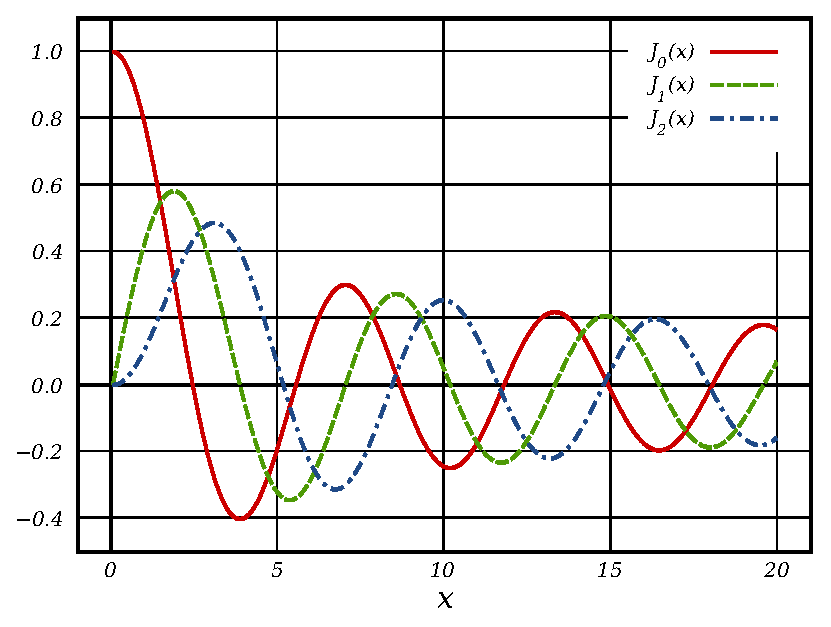
\includegraphics[width=0.5\textwidth]{besselfunctions.eps}
\caption{Bessel-functions source: $ https://de.wikipedia.org/wiki/Besselsche_Differentialgleichung$}
\label{fig:besself}
\end{center}
\end{figure}

We combine the two solutions (\eqref{eq:ansatz05} and \eqref{eq:ansatz06}) for the solution of \eqref{eq:laplcyl}:

\begin{equation}
V=Ce^{-\lambda z}J_0(\lambda r) ~~~,~~~ V=Ce^{\lambda z}J_0(\lambda r) \label{eq:ansatz07}
\end{equation}
$\lambda$ varies from $0$ to $\infty$ and $C$ varies in dependence of $\lambda$. Than we write a general solution of the potential \eqref{eq:laplcyl}:
\begin{equation}
V=\int\limits_{0}^{\infty}\left(\phi(\lambda)e^{-\lambda z}+\psi(\lambda)e^{\lambda z}\right)J_0(\lambda r) d\lambda \label{eq:sol-lapleq}
\end{equation}

Where $\phi(\lambda)$ and $\psi(\lambda)$ are arbitrary functions of $\lambda$.

\subsubsection*{Potential of homogeneous halfspace}
Starting of with the potential in cylindrical coordinates:
\begin{equation}
V=\frac{I\rho}{2\pi\sqrt{r^2+z^2}}\label{eq:2-20}
\end{equation}
Looking at the \textit{Lipschitz-Integral}:
\begin{equation}
\int\limits_{0}^{\infty}e^{-\lambda z}J_0(\lambda r)d\lambda=\frac{1}{\sqrt{r^2+z^2}} \label{eq:lipschitzint}
\end{equation}

Now using \eqref{eq:lipschitzint} we write \eqref{eq:2-20} as:
\begin{equation}
V=\frac{\rho_1 I}{2\pi}\int\limits_{0}^{\infty}e^{-\lambda z}J_0(\lambda r)d\lambda
\end{equation}

The general solution \eqref{eq:sol-lapleq} can now be written:
\begin{equation}
V=\frac{\rho_1 I}{2\pi}\int\limits_{0}^{\infty}\left(e^{-\lambda z}+\theta(\lambda)e^{-\lambda z}+X(\lambda)e^{\lambda z}\right) J_0(\lambda r)d\lambda \label{eq:sol-lapleq-2}
\end{equation}

Where $\theta(\lambda)$ and $X(\lambda)$ are arbitrary functions of $\lambda$, and $\phi(\lambda)=\frac{\rho_1 I}{2\pi}\left(1+\theta(\lambda)\right)$ and $\psi(\lambda)=\frac{\rho_1 I}{2\pi}X(\lambda)$.

The solutions of the form \eqref{eq:sol-lapleq-2} are valid in all layers but $\theta(\lambda)$ and $X(\lambda)$ can be different for each layer $i$:
\begin{equation}
V_i=\frac{\rho_1 I}{2\pi}\int\limits_{0}^{\infty}\left(e^{-\lambda z}+\theta_i(\lambda)e^{-\lambda z}+X_i(\lambda)e^{\lambda z}\right)J_0(\lambda r) d\lambda\label{eq:sol-lapleq-3}
\end{equation}

\subsubsection*{Adaption of the solution to the boundary conditions}

Assuming we are at the layer boundaries of $z=h_i$.


\begin{compactenum}[A)]
\item Potential \eqref{eq:sol-lapleq-3} is continious at each boundary plane in the subsurface:
\begin{equation}
V_i(r,h_i)=V_{i+1}(r,h_i)
\end{equation}
This equation can only be satisfied if the integrands on both sides are equal:
\begin{equation}
\theta_i(\lambda)e^{-\lambda h_i}+X_i(\lambda)e^{\lambda h_i}=\theta_{i+1}(\lambda)e^{-\lambda h_i}+X_{i+1}(\lambda)e^{\lambda h_i} \label{eq:boundary-2-23A}
\end{equation}
\item At each boundary plane $j_z$ the boundary condition must be fulfilled that:
\begin{equation}
j_z=-\frac{1}{\rho}\frac{\partial V}{\partial z}
\end{equation} 
and so
\begin{equation}
\frac{1}{\rho_i}\left(\left(1+\theta_i(\lambda)\right)e^{\lambda h_i}-X_i(\lambda)e^{\lambda h_i}\right)=\frac{1}{\rho_{i+1}}\left(\left(1+\theta_{i+1}(\lambda)\right)e^{\lambda h_i}-X_{i+1}(\lambda)e^{\lambda h_i}\right) \label{eq:boundary-2-23B}
\end{equation}
To satisfy this condition we differentiate the expression for the potential in the first layer \eqref{eq:2-20} with respect to $z$ and then substitute $z=0$:
\begin{equation}
\frac{1}{\rho_1}\frac{\partial V_1(r,0)}{\partial z}=0 ~~~,~ \textrm{for~~} r\neq 0
\end{equation}
We thus obtain the equation:
\begin{equation}
\int\limits_{0}^{\infty}\left(-1-\theta_1(\lambda)+X_1(\lambda)\right) J_0(\lambda_r)d\lambda=0
\end{equation}
\begin{equation}
\Rightarrow \theta_1(\lambda)=X_1(\lambda) \label{eq:boundary-2-23C}
\end{equation}

\item Near the current source the potential must approach to infinity
\begin{align*}
V_\infty=\frac{\rho I}{2\pi}\frac{1}{\sqrt{r^2+z^2}}
\end{align*}
which is approaching asymtotically to the potential for a layer extending to infinite height.

\item $V\rightarrow 0$ if $z\rightarrow\infty$ 
\begin{equation}
\Rightarrow X_n=0 \label{eq:boundary-2-23D}
\end{equation}
, because otherwise $e^{\lambda z}$ would drive the potential to an infinite value at an infinite depth.

\end{compactenum}

The set of equations \eqref{eq:boundary-2-23A} - \eqref{eq:boundary-2-23D} provides a system of $2n$ equation in $2n$ unknown functions $\theta(\lambda)$ and $X(\lambda)$. To obtain the solution subsitute \eqref{eq:boundary-2-23C} into \eqref{eq:boundary-2-23A} and \eqref{eq:boundary-2-23B} and subsitute \eqref{eq:boundary-2-23D} into \eqref{eq:boundary-2-23A} and \eqref{eq:boundary-2-23B}.

For brevity, we introduce the notations:
\begin{align*}
u_i=e^{\lambda h_i}, v_i=\frac{1}{u_i}, p_i=\frac{\rho_i}{\rho_{i+1}}
\end{align*}
The system of equations then become:
\begin{align*}
(u_1+v_1)\theta_1-u_2\theta_2-v_2X_2&=0\\
(v_1-u_1)\theta_1+p_1u_1\theta_2-p_1v_1X_2&=(1-p_1)u_1\\
\vdots~~~~~~~~~~~~~~~~~~~~&\vdots\\
u_{n-1}\theta_{n-1}+v_{n-1}X_{n-1}-u_{n-1}\theta_n&=0\\
-u_{n-1}\theta_{n-1}+v_{n-1}X_{n-1}+p_{n-1}u_{n-1}\theta_n-p_{n-1}v_{n-1}X_n&=(1-p_{n-1})u_{n-1}
\end{align*}
Solution of the equations by applying \textit{Cramer's rule}. For example: Solution of a two layer case (layer 1: $\rho_1, h_1$, layer 2: $\rho_2$):
\begin{align*}
\theta_1&=\frac{ku}{1-ku} && \theta_2=\frac{k(1+u)}{1-ku}\\
X_1&=\theta_1 && X_2=0
\end{align*}
with $u=e^{-2\lambda h_1}$ and the \textit{reflection coefficient of DC} $k=\frac{\rho_2-\rho_1}{\rho_2+\rho_1}$

Interesting is the potential at the surface of the earth, with $z=0$ and \eqref{eq:boundary-2-23C}:
\begin{align}
V_0=V_1(r,z)&=\frac{\rho_1 I}{2\pi}\int\limits_{0}^{\infty}\left(1+2\theta_1\right)J_0(\lambda r)d\lambda\\
&=\frac{\rho_1 I}{2\pi}\int\limits_{0}^{\infty}K(\lambda)J_0(\lambda r)d\lambda
\end{align}
where $K(\lambda)$ is the \textit{Slichter-function}.

We consider the Lipschitz-integral:
\begin{equation}
\int\limits_{0}^{\infty}e^{-\lambda z}J_0(\lambda r)d\lambda=\frac{1}{\sqrt{r^2+z^2}}\stackrel{i=0}= \int\limits_{0}^{\infty}J_0(\lambda r)d\lambda=\frac{1}{r}
\end{equation}
\eqref{eq:sol-lapleq-3} can now be written in the form:
\begin{equation}
V_0(r)=\underbrace{\frac{I}{2\pi}\left(\frac{\rho_1}{r}\right.}_{\textrm{first layer}}\left.+\int\limits_{0}^{\infty}(T(\lambda)-\rho_1)J_0(\lambda r)d\lambda\right)
\end{equation}

Example/reminder for four point measurement:
\begin{align*}
V_1=\frac{I\rho}{2\pi}\left(\frac{1}{AM}-\frac{1}{BM}\right)
\end{align*}

\subsubsection{Derivation of a formula for the apparent resistivity}
Take an arbitrary DC-Array (compare Fig. \ref{fig:dc01}). Then
\begin{align*}
\Delta U=\frac{I\rho}{2\pi}\left(\frac{1}{AM}-\frac{1}{AN}-\frac{1}{BM}+\frac{1}{BN}\right)
\end{align*}
\begin{align*}
\rho_a=k\frac{\Delta U}{I}
\end{align*}
where $k$ is the geometrical factor.
If we look at experimental data with an error of 1\% for the distances between the electrodes, the error in $\rho_a$ would be 2\%. But 10\% error in the lateral direction of the electrodes results only in 1\% error in $\rho_a$.

In case of the Schlumberger array ($L=AM+MN/2$ and $a=MN$, $a\ll L$) we get a voltage decrease in U:
\begin{align*}
U&=2\left(V_0(\frac{L}{2}-\frac{a}{2}\right)-V_0\left(\frac{L}{2}+\frac{a}{2}\right)\\
&\approx -2a\frac{\partial V_0}{\partial r}\bigg|_{r=L/2}
\end{align*}
and the geometrical factor in case of Schlumberger $k=\frac{\pi}{a}\left(\left(\frac{L}{2}\right)^2-\left(\frac{a}{2}\right)^2\right)$
\begin{align*}
\rho_a(L/2)=K\frac{U}{I}=\frac{2\pi}{I}\left(\frac{L}{2}\right)^2\frac{\partial V_0}{\partial r}
\end{align*}
with $\frac{d}{dx}J_0(x)=-J_1(x)$. From eq. 2.25!!!!:

\begin{equation}
\rho_a(L/2)=\rho_1+\left(\frac{L}{2}\right)^2\underbrace{\int\limits_{0}^{\infty}(T(\lambda)-\rho_1)J_1(\lambda L/2)\lambda d\lambda}_{\textrm{Stefanescu-Integral}} \label{eq:rho_a_01}
\end{equation}

The calculations of the model response $\rho_a(L/2)$ from given model parameters $(\rho_i,h_i)$ is a forward problem. 

Given:
\begin{figure}[h!]
\begin{center}
\caption{Given parameters}
\label{fig:forwardgiven}
\end{center}
\end{figure}
